%%%%%%%%%%%%%%%%%%%%%%%%%%%%%%%%%%%%%%%%%
% Short Sectioned Assignment
% LaTeX Template
% Version 1.0 (5/5/12)
%
% This template has been downloaded from:
% http://www.LaTeXTemplates.com
%
% Original author:
% Frits Wenneker (http://www.howtotex.com)
%
% License:
% CC BY-NC-SA 3.0 (http://creativecommons.org/licenses/by-nc-sa/3.0/)
%
%%%%%%%%%%%%%%%%%%%%%%%%%%%%%%%%%%%%%%%%%

%----------------------------------------------------------------------------------------
%	PACKAGES AND OTHER DOCUMENT CONFIGURATIONS
%----------------------------------------------------------------------------------------

\documentclass[paper=a4, fontsize=11pt]{scrartcl} % A4 paper and 11pt font size
\usepackage{braket}
\usepackage[T1]{fontenc} % Use 8-bit encoding that has 256 glyphs
\usepackage{graphicx}
\usepackage{float}
\usepackage[english]{babel} % English language/hyphenation
\usepackage{amsmath,amsfonts,amsthm} % Math packages
\usepackage{subcaption}
\usepackage{sectsty} % Allows customizing section commands
\allsectionsfont{\centering \normalfont\scshape} % Make all sections centered, the default font and small caps
\usepackage{hyperref}
\usepackage[utf8]{inputenc}
\usepackage{fancyhdr} % Custom headers and footers
\pagestyle{fancyplain} % Makes all pages in the document conform to the custom headers and footers
\fancyhead{} % No page header - if you want one, create it in the same way as the footers below
\fancyfoot[L]{} % Empty left footer
\fancyfoot[C]{} % Empty center footer
\fancyfoot[R]{\thepage} % Page numbering for right footer
\renewcommand{\headrulewidth}{0pt} % Remove header underlines
\renewcommand{\footrulewidth}{0pt} % Remove footer underlines
\setlength{\headheight}{13.6pt} % Customize the height of the header

\numberwithin{equation}{section} % Number equations within sections (i.e. 1.1, 1.2, 2.1, 2.2 instead of 1, 2, 3, 4)
\numberwithin{figure}{section} % Number figures within sections (i.e. 1.1, 1.2, 2.1, 2.2 instead of 1, 2, 3, 4)
\numberwithin{table}{section} % Number tables within sections (i.e. 1.1, 1.2, 2.1, 2.2 instead of 1, 2, 3, 4)

\setlength\parindent{0pt} % Removes all indentation from paragraphs - comment this line for an assignment with lots of text



%----------------------------------------------------------------------------------------
%	TITLE SECTION
%----------------------------------------------------------------------------------------

\newcommand{\horrule}[1]{\rule{\linewidth}{#1}} % Create horizontal rule command with 1 argument of height

\title{	
\normalfont \normalsize 
\textsc{Algorithmic Methods of Data Mining and Laboratory} \\ [25pt] % Your university, school and/or department name(s)
\textsc{Sapienza Università di Roma} \\ [25pt]
\horrule{0.5pt} \\[0.4cm] % Thin top horizontal rule
\huge Search Engine\\ % The assignment title
\horrule{2pt} \\[0.5cm] % Thick bottom horizontal rule
}
\author{S. Ballesteros\footnote{sergio.ballesteros@estudiante.uam.es} , F. Crema\footnote{email} , G. Nespoli\footnote{email}} % Your name

\date{\normalsize\today} % Today's date or a custom date

\begin{document}

\maketitle % Print the title

%----------------------------------------------------------------------------------------
%	PROBLEM 1
%----------------------------------------------------------------------------------------

\section{Introduction}
Here we present a search engine writen in Python that is capable of indexing the information of the more than 11 000 recipes available at the \href{http://www.bbc.co.uk/food/recipes/}{BBC  food section webpage} and showing the most relevant results when searching a query through its graphical interface. \\
In the following sections we describe the differents parts our work, as well as its authors: Information download, Preprocessing, Search engine and Graphical Interface.

\section{Information download}
The purpose of this part is to download as many recipes as possible from de BBC webpage, and to parse the relevant information to a TSV file. The proccess is as follows:
\subsection{Finding the recipes links}
The python module of this part is stored in \textit{search/download/downloadData.py}. All the recipes links begin by \textit{http://www.bbc.co.uk/food/recipes/}, in order to find those links, we investigated two sections of the BBC webpage, the first one is the ingredient section, and the second one is their own search tool. \\\
\subsubsection{Ingredients section}
Since each ingredient webpage link to several link recipes, we found the links to the ingredients webpages. In order to do so, our Python programm analyzes the following set of webpages \textit{http://www.bbc.co.uk/food/ingredients/by/letter/[a-z]/} and then parses all the links that has the form \textit{http://www.bbc.co.uk/food/[ingredient]}, which lead to the [ingredient] page. \\ \\
After getting all the ingredient links, our programm explores each ingredient page to find the recipes links, which have the format \textit{http://www.bbc.co.uk/food/recipes/[recipe]}. Both the links to the discovered recipes and the already explored ingredients are saved on the fly to two files on the disk. In this way, if the process is interrupted, the program can be ran again and by default it will load those files to resume the process in the point where it stopped.

\begin{figure}[H]
\centering
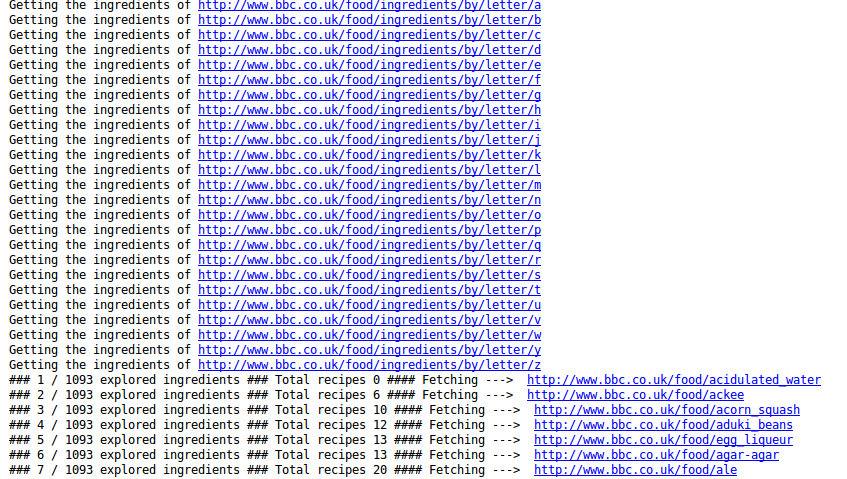
\includegraphics[width=1\textwidth]{images/downloadslinks}
\caption{Our program output: in the top the program is finding the links to the ingredients webpages, and in the bottom is finding the link to the recipes inside each ingredient webpage.}
\end{figure}

Only about 5 000 recipies links can be found exploring directly the ingredients. On the other hand, on the BBC webpage, it is anounced that there are more than 11 000 recipes available. To our knowledge, the only way to find all of them is to use the search engine of the own webpage. In order to do so, we sent petitions to the webpage of the format \textit{http://www.bbc.co.uk/food/recipes/search?keywords=[ingredient]\&page=[page number]}, where [page number] ranges from 1 to a maximum number that we parsed also from the page 1. The following image shows where to get this links, although our program created the set of all links in the mentioned format using as a base the links that the webpagesent us.

\begin{figure}[H]
\centering
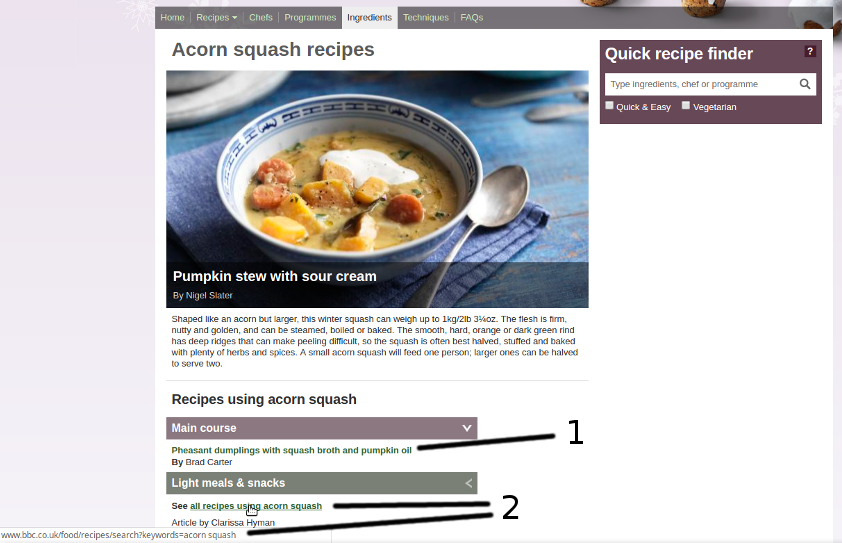
\includegraphics[width=0.9\textwidth]{images/ingredient}
\caption{Sample ingredient webpage with: 1. Direct link to a recipe, 2. link to the search engine of the BBC webpage with a sample query.}
\end{figure}

\subsubsection{Built in search engine}

\begin{figure}[H]
\centering
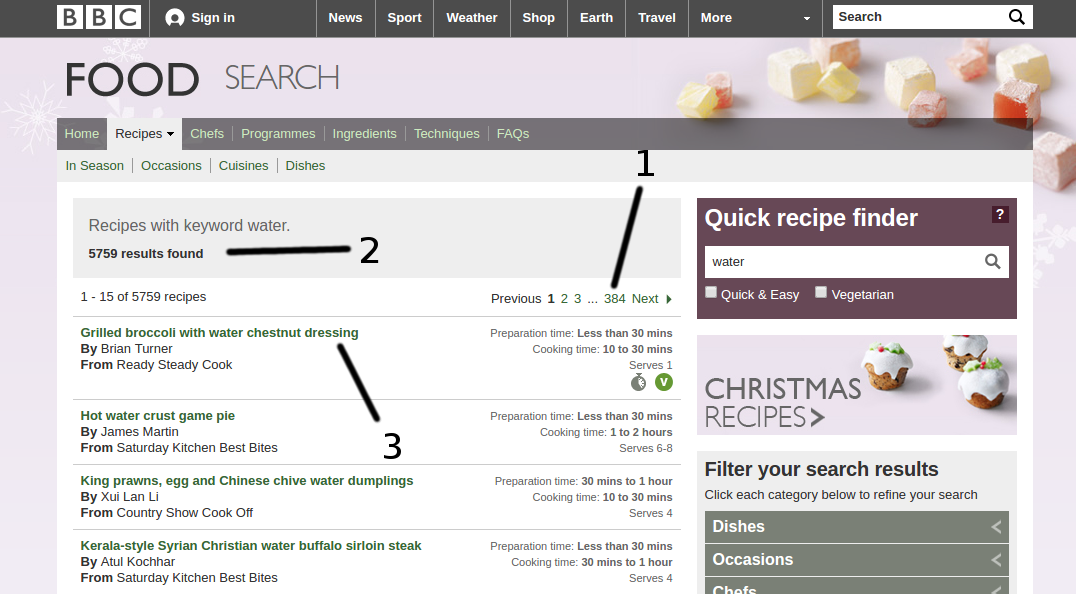
\includegraphics[width=1\textwidth]{images/search}
\caption{Example of the query \textit{water} under the webpage search functionality with: 1. Maximum number of pages, 2. Total number of recipes under this query, 3. Example of one recipe link}
\end{figure}

Then the program explored each search webpage until found all the recipes, which by the time when we ran it were 11 224 recipes. \\
Also an other feature of our program is that it retries to get the webpage up to 3 times, with 5 seconds pause in between petitions. If still the information can not be retrieved, the link is saved to be explored the next time that the program is ran. We also made sure that the links were not explored twice and the links to the recipes were unique using sets to store them in memory before writing them to disk. 

\subsection{Analyzing the recipes}
 The python module of this part is stored in \textit{search/download/analyzeRecipes.py}. In this part the information of each recipe is saved on the fly to a TSV file in disk that can be found in data/data.tsv. The extracted information of each recipe is the recipe name, author name, programme name, preparation time, cooking time, number of serves, URL of the picture, method of cooking, ingredients, vegetarian or not, caloric content (in kcal), grams of protein, carb, sugar, fat, saturated fat, fiber, salt. When the values where missing, the missing value was replaced by \textit{NaN}. In order to do so we made use of the built in functionality of Python for managing errors \textit{try}.
 
\begin{figure}[H]
\centering
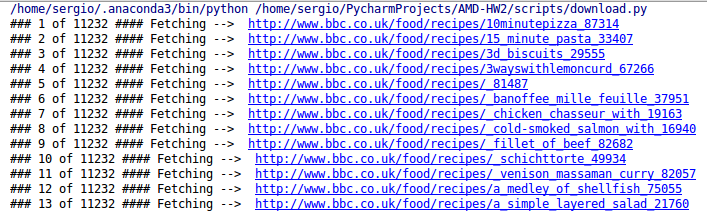
\includegraphics[width=1\textwidth]{images/analyze}
\caption{Example of extracting the information of the recipes.}
\end{figure}

\subsection{How to run the program to download the recipes}

The script to execute is located in \textit{scripts/download.py}. The working directory should be set to the root folder. If the script is ran by default, it will find more recipes and analize them, updating the file \textit{data.tsv}. On the other hand, if we want to find all the recipes from scratch, we have to ran the script setting the variables that we will find inside to \textit{reset = True}. Right after that, we should change the variables \textit{reset} again to False to make use of the feature of continue exploring the links and the recipes from the interrupted point without erasing again the stored files.







\section{Preprocessing}
\section{Search engine}
\section{Graphical interface}




\end{document}
